\documentclass[12pt]{article}
\usepackage{times}
\usepackage[utf8]{inputenc}
\usepackage[T2A,T1]{fontenc}
\usepackage[caption]{caption}
\usepackage{amsmath}
\usepackage{amsfonts}
\usepackage{amssymb}
\usepackage[version=4]{mhchem}
\usepackage{stmaryrd}
\usepackage[russian]{babel}
\usepackage{geometry}
\usepackage{lmodern}
\usepackage{graphicx}
\usepackage[export]{adjustbox}
\usepackage[pdfborder={0 0 0}]{hyperref}
\usepackage{algorithm}
\usepackage{algpseudocode}
\usepackage{float}

% Геометрия страницы
\geometry{
  top=2cm,
  bottom=2cm,
  left=2.5cm,
  right=1cm
}

% Отступ красной строки
\setlength{\parindent}{1.25cm}

% Междустрочный интервал
\renewcommand{\baselinestretch}{1.5}

\renewcommand{\figurename}{Рисунок}

\begin{document}

\begin{titlepage}
\newcommand{\HRule}{\rule{\linewidth}{0.2mm}}

\begin{center}
\textsc{ \centering МИНИСТЕРСТВО НАУКИ И ВЫСШЕГО ОБРАЗОВАНИЯ РОССИЙСКОЙ ФЕДЕРАЦИИ
Федеральное государственное автономное образовательное учреждение высшего образования
«САНКТ-ПЕТЕРБУРГСКИЙ ГОСУДАРСТВЕННЫЙ УНИВЕРСИТЕТ
АЭРОКОСМИЧЕСКОГО ПРИБОРОСТРОЕНИЯ»}\\[0.2cm]
\textsc{КАФЕДРА 25}\\[1cm]
\end{center}

ПРЕПОДАВАТЕЛЬ

\begin{table}[h]
\begin{center}
\begin{tabular}{|c|c|c|}
\hline
Доцент к.т.н. & 27.12.2024 & Е. М. Линский\\
\hline
должность, уч. степень, звание & подпись, дата & инициалы, фамилия\\
\hline
\end{tabular}
\end{center}
\end{table}

\begin{center}
\textsc{\Large{ОТЧЁТ ПО КУРСОВОЙ РАБОТЕ}}\\[0.5cm]
\textsc{\Large{''АЛГОРИТМ ФАНО''}}\\[2cm]
\textsc{по курсу: ОСНОВЫ ПРОГРАММИРОВАНИЯ}\\[3cm]
\end{center}

РАБОТУ ВЫПОЛНИЛ

\begin{table}[h]

\begin{center}
\begin{tabular}{|c|c|c|c|}
\hline
Студент гр. № & 2352 & 27.12.2024& Т. А. Потапов\\
\hline
& & подпись, дата & инициалы, фамилия \\
\hline
\end{tabular}
\end{center}
\end{table}

\begin{center}
{\large Санкт-Петербург 2024}
\end{center}
\end{titlepage}


% Оглавление
\tableofcontents
\newpage

% Постановка задачи
\section{\textbf{ПОСТАНОВКА ЗАДАЧИ}}
Задачей данной курсовой работы является разработка программы для кодирования и декодирования файлов с использованием алгоритма Шеннона-Фано. Программа должна предоставлять возможность архивировать одиночные текстовые файлы, сжимая их размер, а затем восстанавливать их до исходного состояния.

Программа реализует алгоритм Фано, который основывается на разбиении символов исходного текста на группы, исходя из их частот, и присвоении им уникальных префиксных кодов.

\subsection*{Свойства алгоритма Фано:}
\begin{itemize}
    \item Кодирование должно быть префиксным, чтобы обеспечить однозначность декодирования.
    \item Часто встречающиеся символы получают более короткие коды, реже встречающиеся — более длинные.
    \item Программа должна эффективно обрабатывать текст с произвольным количеством символов.
\end{itemize}

\textbf{Пример задачи:} Дан текстовый файл с содержимым \texttt{hello world}. Программа должна сжать его, создав закодированный файл и сопутствующий словарь кодов. После разархивации из сжатого файла должен быть восстановлен исходный текст.

\textbf{Литература:} М.Н. Аршинов, Л.Е. Садовский, Коды и математика, Издательство: «Наука», 1996.

% Описание алгоритма
\newpage
\section{\textbf{ОПИСАНИЕ АЛГОРИТМА}}
\subsection{Основные идеи алгоритма}
Алгоритм Шеннона-Фано основан на следующих концепциях:
\begin{enumerate}
    \item Символы сортируются по убыванию частоты их появления.
    \item Множество символов разбивается на две группы с примерно равной суммарной частотой.
    \item К первой группе добавляется бит 0, ко второй — 1.
    \item Процесс повторяется рекурсивно для каждой группы, пока все символы не будут закодированы.
\end{enumerate}

\captionsetup[figure]{labelfont=bf, labelsep=endash}

\subsection{Подробное описание алгоритма}
\begin{enumerate}
    \item \textbf{Сбор статистики:} анализируется входной текст, и подсчитывается частота каждого символа.
    \item \textbf{Сортировка символов:} символы сортируются по частоте в порядке убывания.
    \item \textbf{Построение кодов:} применяется рекурсивный метод, описанный выше.
        \begin{figure}[H]
        \centering
            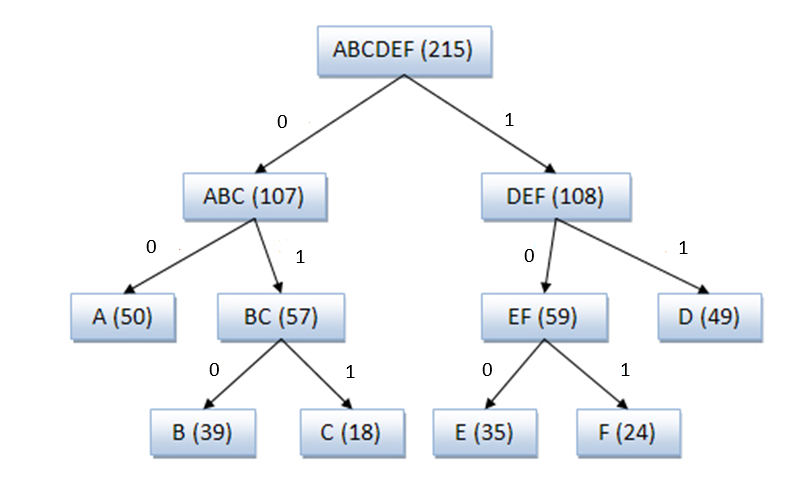
\includegraphics[scale=0.5]{temp.png}
            \caption{Пример построения кодов}
        \end{figure}
         
    \item \textbf{Создание словаря:} генерируется отображение символов в их коды.
    \item \textbf{Кодирование текста:} каждый символ текста заменяется соответствующим кодом.
    \item \textbf{Декодирование:} используя словарь, сжатый текст преобразуется обратно в исходный.
\end{enumerate}

\subsection{Пример выполнения алгоритма}
Шаги алгоритма для текста \texttt{abacabad}:
\begin{enumerate}
    \item Частоты символов: $a: 4, b: 2, c: 1, d: 1$.
    \item Сортировка: $a (4), b (2), c (1), d (1)$.
    \item Разбиение: \begin{itemize}
        \item Первая группа: $a (4) \to$ код 0.
        \item Вторая группа: $b (2), c (1), d (1) \to$ код 1.
    \end{itemize}
    \item Рекурсивное разбиение второй группы:
        \begin{itemize}
            \item $b (2) \to$ код 10.
            \item $c (1), d (1) \to$ код 11.
        \end{itemize}
    \item Итоговые коды: $a: 0, b: 10, c: 110, d: 111$.
    \item Кодирование текста: \texttt{abacabad} $\to 010011010111$.
\end{enumerate}

\subsection{Псевдокод алгоритма}
\begin{algorithm}[H]
\caption{Анализ текста для подсчета частот символов}
\begin{algorithmic}[1]
\Function{analyzeText}{текст}
    \State Создать словарь частот символов
    \For{каждый символ в тексте}
        \If{символ пробел}
            \State Увеличить счётчик частоты для "\texttt{\textbackslash x20}"
        \ElsIf{символ новая строка}
            \State Увеличить счётчик частоты для "\texttt{\textbackslash n}"
        \Else
            \State Увеличить счётчик частоты для строки, содержащей этот символ
        \EndIf
    \EndFor

    \For{каждая пара символ-частота в словаре}
        \State Добавить символ с его частотой в список символов
    \EndFor

    \State Отсортировать список символов по убыванию частот
    \State Вызвать \Call{buildCodes}{0, размер списка символов - 1}
    \State Построить словари для кодировки и декодировки символов
\EndFunction
\end{algorithmic}
\end{algorithm}

\begin{algorithm}[H]
\caption{Рекурсивное построение кодов для символов}
\begin{algorithmic}[1]
\Function{buildCodes}{начало, конец}
    \If{начало >= конец}
        \State Завершить выполнение функции
    \EndIf

    \State totalFrequency = 0
    \For{i от начало до конец}
        \State totalFrequency += частота символа[i]
    \EndFor

    \State halfFrequency = 0
    \State splitIndex = начало
    \For{i от начало до конец}
        \State halfFrequency += частота символа[i]
        \If{halfFrequency >= totalFrequency / 2}
            \State splitIndex = i
            \State Прервать цикл
        \EndIf
    \EndFor

    \For{i от начало до splitIndex}
        \State Добавить "0" в код символа[i]
    \EndFor

    \For{i от splitIndex + 1 до конец}
        \State Добавить "1" в код символа[i]
    \EndFor

    \State \Call{buildCodes}{начало, splitIndex}
    \State \Call{buildCodes}{splitIndex + 1, конец}
\EndFunction
\end{algorithmic}
\end{algorithm}

\newpage
\subsection{\textbf{Aнализ сложности алгоритма}}

\begin{enumerate}
    \item Подсчет частот символов: \textbf{Сложность}: $O(n)$
    \item Перенос частот в список: \textbf{Сложность}: $O(k)$
    \item Сортировка списка: \textbf{Сложность}: $O(k \log k)$
    \item Построение кодов (рекурсивно): \textbf{Сложность}: $O(k \log k)$
\end{enumerate}

Итоговая сложность: $O(n + k \log k)$

\begin{itemize}
    \item Если $n \gg k$, то сложность $O(n)$, так как обработка текста доминирует.
    \item Если $k \gg \log k$, то сложность $O(k \log k)$.
\end{itemize}

\newpage
% Инструкция пользователя
\section{\textbf{ИНСТРУКЦИЯ ПОЛЬЗОВАТЕЛЯ}}
\noindent
\textbf{1. Запуск программы:}
\begin{verbatim}
./ShanonFano <режим> <входной файл> <выходной файл>
\end{verbatim}
\begin{itemize}
    \item $<$режим$>$: encode для сжатия или decode для разархивации.
    \item $<$входной файл$>$: имя файла для обработки.
    \item $<$выходной файл$>$: имя файла для сохранения результата.
\end{itemize}

\noindent
\textbf{2. Формат входного файла:}
\begin{itemize}
    \item \textbf{Режим encode:} Текстовый файл с любым содержимым. Поддерживаются пробелы и переносы строк.
    \item \textbf{Режим decode:} Бинарный файл с закодированными данными.
\end{itemize}

\noindent
\textbf{3. Формат выходного файла:}
\begin{itemize}
    \item \textbf{Режим encode:} Бинарный файл с закодированными данными, текстовый файл со словарем символов.
    \item \textbf{Режим decode:} Текстовый файл с восстановленным содержимым.
\end{itemize}

\newpage
% Тестовые примеры
\section{\textbf{ТЕСТОВЫЕ ПРИМЕРЫ}}
\begin{enumerate}
    \item \textbf{Тест 1:}
    \begin{itemize}
        \item Ссылка на текст: \url{https://www.gutenberg.org/cache/epub/12299/pg12299.txt}
        \item Вес текста до архивации: 385 KB
        \item Вес текста после архивации: 221 KB
    \end{itemize}
    \item \textbf{Тест 2:}
    \begin{itemize}
        \item Ссылка на текст: \url{https://www.gutenberg.org/cache/epub/12299/pg12299.txt}
        \item Вес текста до архивации: 280 KB
        \item Вес текста после архивации: 169 KB
    \end{itemize}
    \item \textbf{Тест 3:}
    \begin{itemize}
        \item Ссылка на текст: \url{https://www.gutenberg.org/cache/epub/80/pg80.txt}
        \item Вес текста до архивации: 620 KB
        \item Вес текста после архивации: 371 KB
    \end{itemize}
\end{enumerate}

\newpage
% Список литературы
\section{\textbf{СПИСОК ЛИТЕРАТУРЫ}}
\begin{enumerate}
    \item М. Н. Аршинов, Л. Е. Садовский, Коды и математика (рассказы о кодировании).- М.: Наука, Главная редакция физико-математической литературы, 1983. - 144 с.
    \item Алгоритм Шеннона-Фано. // Алгоритмы: электронные текстовые данные, URL: \url{https://habr.com/ru/articles/137766/}, Год публикации: 2012. Режим доступа: открытый. Дата обращения к источнику: 18.12.2024
\end{enumerate}


\end{document}
